\documentclass[a4paper,11pt]{article}
\usepackage[big]{layaureo}
\usepackage[T1] {fontenc}
\usepackage[utf8]{inputenc}
\usepackage[italian] {babel}
\usepackage{textcomp}
\usepackage{amsmath}
\usepackage{amssymb}
\usepackage{graphicx}
\usepackage{multirow}
\usepackage{caption}
  \captionsetup{format=hang,labelfont=bf,textfont=it, font=small}
\usepackage{subcaption}
  \captionsetup[sub]{position=top}
  \captionsetup[sub]{font=footnotesize}
  \captionsetup[sub]{labelfont={bf,sc}}
\usepackage{booktabs}
\usepackage{tabularx}
\usepackage{siunitx}
\usepackage{color}
\usepackage{float}
\usepackage{comment}
\usepackage{verbatim}
\usepackage{listings}

\title{MAPD mod. A - Progetto Finale}
\author{Agostini Federico, Bottaro Federico, Pompeo Gianmarco}

\date{18 Ottobre 2019}

\begin{document}

\maketitle

%%%%%%%%%%%%%%%%%%%%%%%%%%%%%%%%%%%%%%%%%%%%%%%%%%
\section{Rappresentazione grafica del progetto}
A scopo introduttivo, riportiamo una schematica di quello che risulterà essere il circuito costruito per il progetto finale.
\begin{figure}[H]
    \centering
    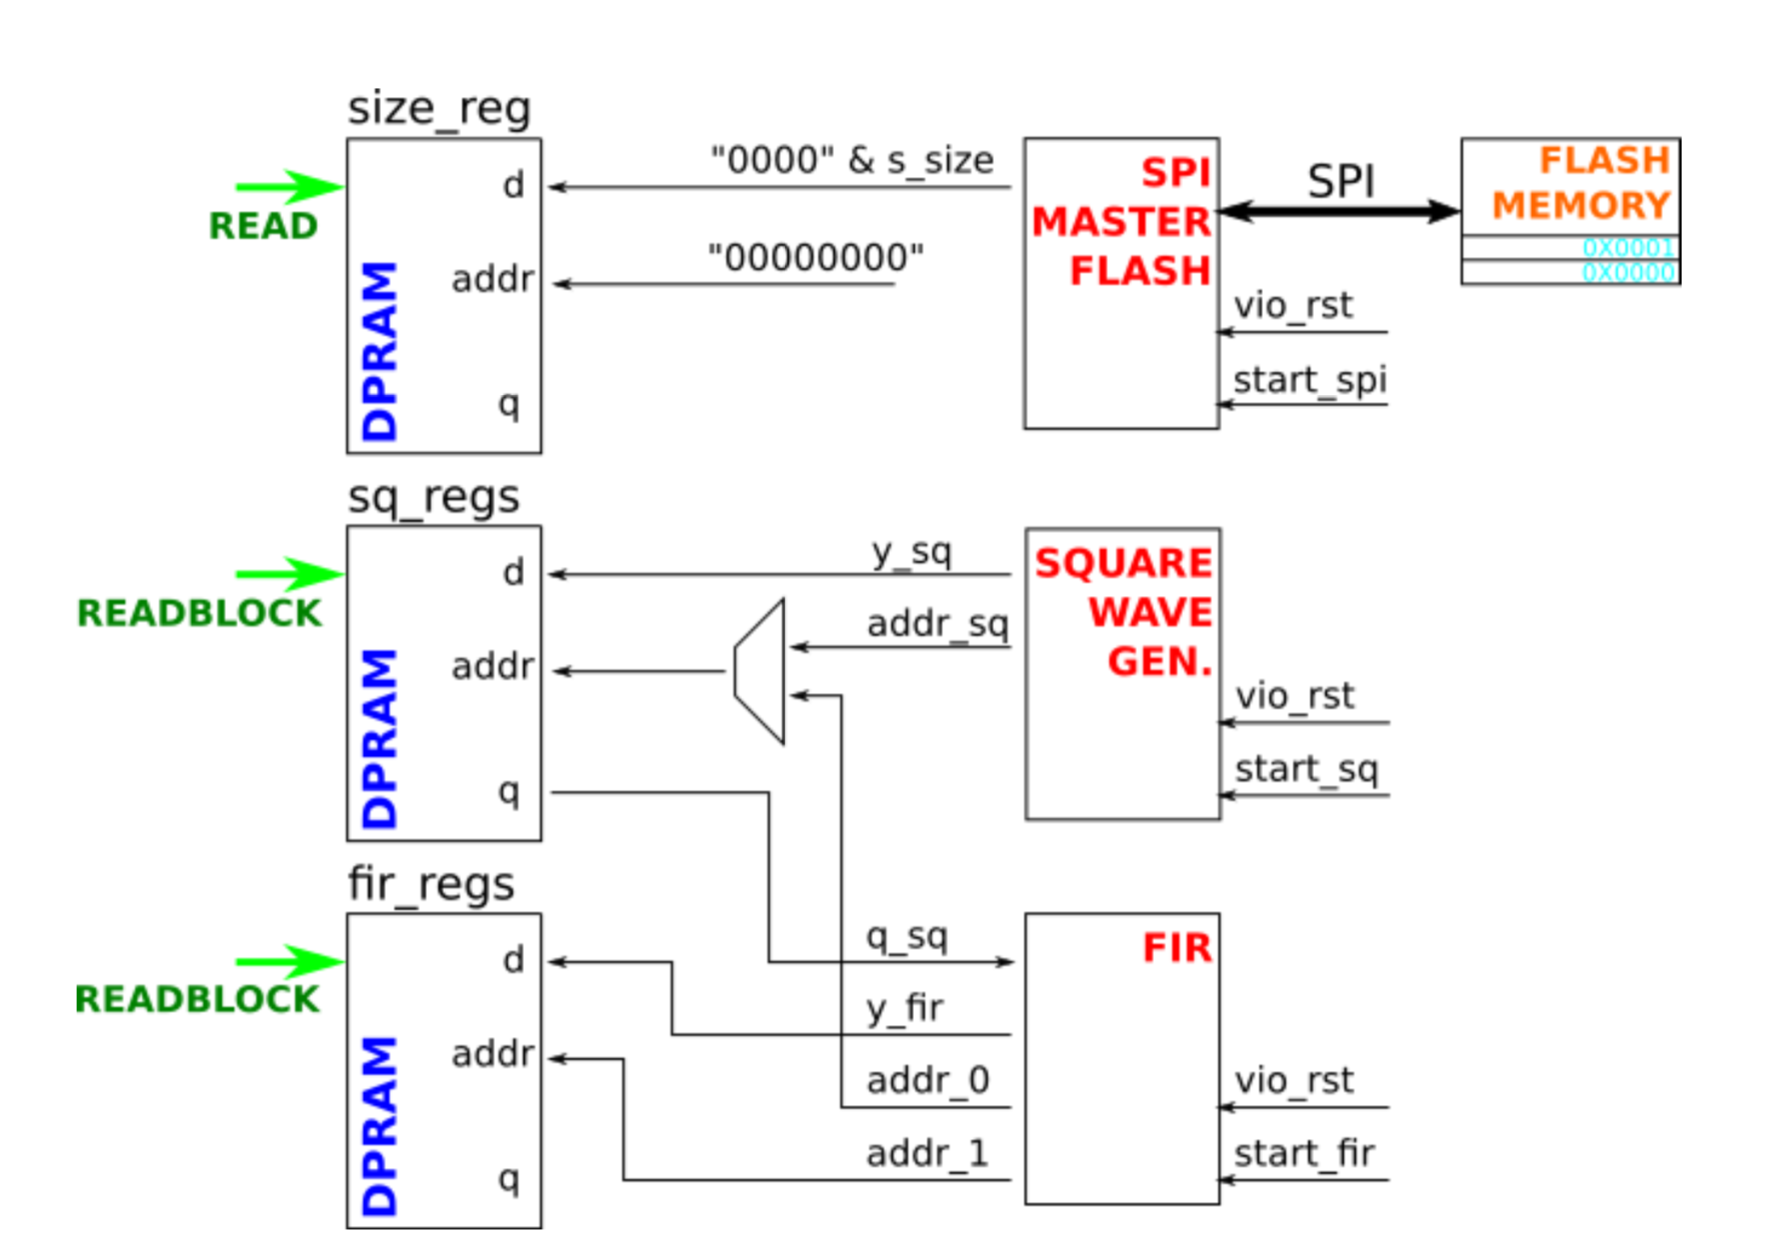
\includegraphics[width=1\textwidth]{./Figure/scheme.png}
    \caption{Schema dei blocchi del circuito implmentato per il progetto finale.}
    \label{fig:scheme}
\end{figure}

%%%%%%%%%%%%%%%%%%%%%%%%%%%%%%%%%%%%%%%%%%%%%%%%%%
\section{VIO policy}
Il VIO (Virtual Input Output) è stato implementato utilizzando tre input virtuali. In particolare, tali input si riferiscono al segnale di reset, al segnale di start connesso al generatore di onda quadra e al segnale di start connesso al filtro FIR. 
\\
Al fine di una corretta esecuzione del software è necessario avviare dapprima il generatore di onda quadra e, dopo qualche istante, procedere con lo start del FIR e lanciare allora gli script in Python per ottenere i grafici desiderati.

%%%%%%%%%%%%%%%%%%%%%%%%%%%%%%%%%%%%%%%%%%%%%%%%%%
\section{Codice \texttt{VHDL}}
Come richiesto, vengono qui riprodotti gli \emph{snippets} di codice in VHDL contenenti le porzioni più salienti del progetto in esame.

%%%%%%%%%%%%%%%%%%%%%%%%%
\subsection{FSM in \texttt{spi\_master\_flash.vhd}}
Nella FSM (Finite State Machine), solo lo stato \texttt{s\_buildword} è stato modificato; si riporta di seguito il codice relativo.

\lstinputlisting[language=VHDL, basicstyle=\footnotesize, numbers=left, numbersep=10pt, numberstyle=\tiny\color{gray}]{./Code/spi_master_flash.txt}

%%%%%%%%%%%%%%%%%%%%%%%%%
\subsection{Generatore di onda quadra: \texttt{low-state}}
Come ultima sezione rilevante, riportiamo lo stato \texttt{low-state} della FSM utilizzata per implementare il generatore di onda quadra; esso corrisponde, come è evidente, allo stato in cui l'onda quadra assume il suo valore minimo.
\lstinputlisting[language=VHDL, basicstyle=\footnotesize, numbers=left, numbersep=10pt, numberstyle=\tiny\color{gray}]{./Code/square_wave.txt}

%%%%%%%%%%%%%%%%%%%%%%%%%
\subsection{FSM nell'\emph{architecture} del FIR}
All'interno dell'architettura del filtro FIR è contenuta una FSM; essa viene riportata di seguito.

\lstinputlisting[language=VHDL, basicstyle=\footnotesize, numbers=left, numbersep=10pt, numberstyle=\tiny\color{gray}]{./Code/fir.txt}

%%%%%%%%%%%%%%%%%%%%%%%%%
\subsection{Implementazione del MUX}
Di seguito riportiamo il codice relativo all'implementazione del MUX (multiplexer).
\\
I tre segnali di input corrispondono ad un indirizzo di memoria proveniente dal generatore di onda quadra e ad un secondo indirizzo generato dal filtro FIR. A questi si aggiunge un terzo input, costituito da un selettore che permette di decidere quale dei due precedenti segnali trasmettere.

\lstinputlisting[language=VHDL, basicstyle=\footnotesize, numbers=left, numbersep=10pt, numberstyle=\tiny\color{gray}]{./Code/mux21.txt}

%%%%%%%%%%%%%%%%%%%%%%%%%%%%%%%%%%%%%%%%%%%%%%%%%%
\section{Filtro FIR}
Sono riportate di seguito le figure ottenute dallo script Python fornitoci. Esse raffigurano nel piano Ampiezza-Frequenza il filtro FIR (Finite Impulse Response) che è stato implementato.

\begin{figure}[htp]
    \centering
    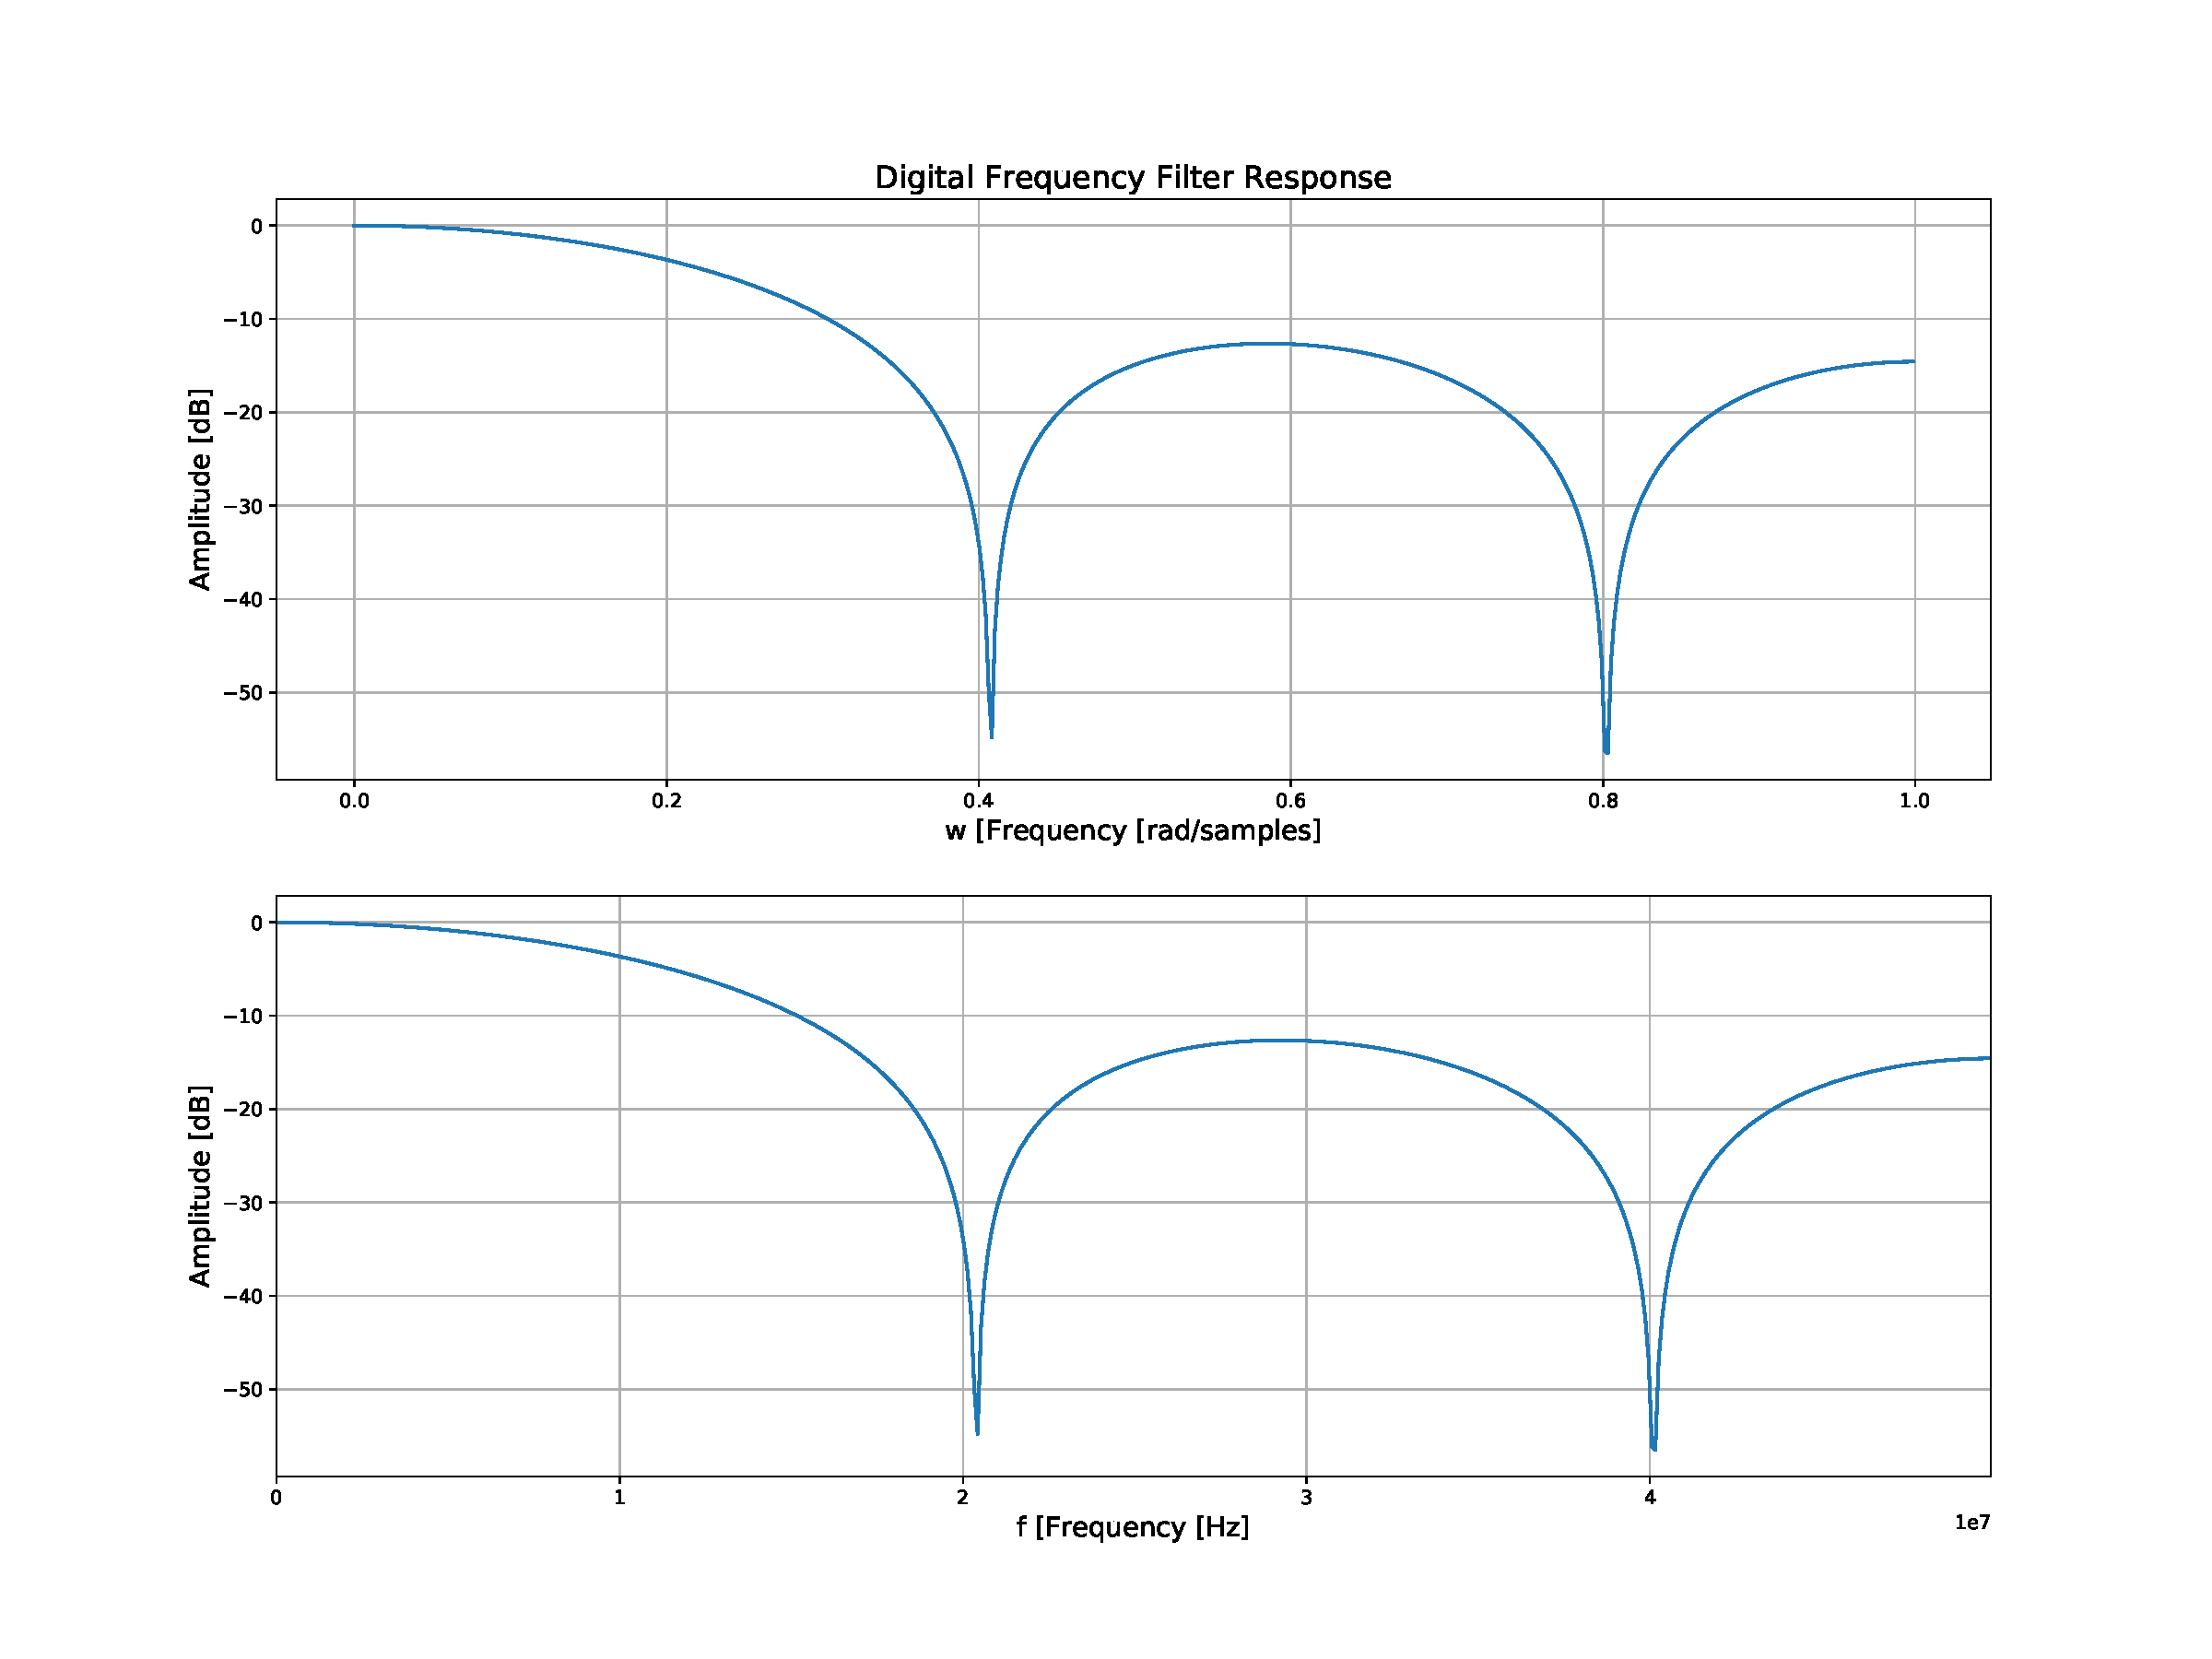
\includegraphics[width=.9\textwidth]{./Figure/f_response.pdf}
    \caption{Immagine prodotta dallo script \texttt{coeff.py} relativa al filtro FIR.}
    \label{fig:filter}
\end{figure}

%%%%%%%%%%%%%%%%%%%%%%%%%%%%%%%%%%%%%%%%%%%%%%%%%%
\newpage
\section{Segnale generato e filtrato}
Di seguito vengono riportate le figure prodotte dallo script \texttt{final\_project.py} in Python al variare dei parametri \texttt{PERIOD} and \texttt{DUTY\_CIC}.

\begin{figure}[H]
    \centering
    \label{fig:plots}
    \begin{subfigure}{0.49\textwidth}
     \caption{\texttt{PERIOD} = 20, \texttt{DUTY\_CYC} = 50}
      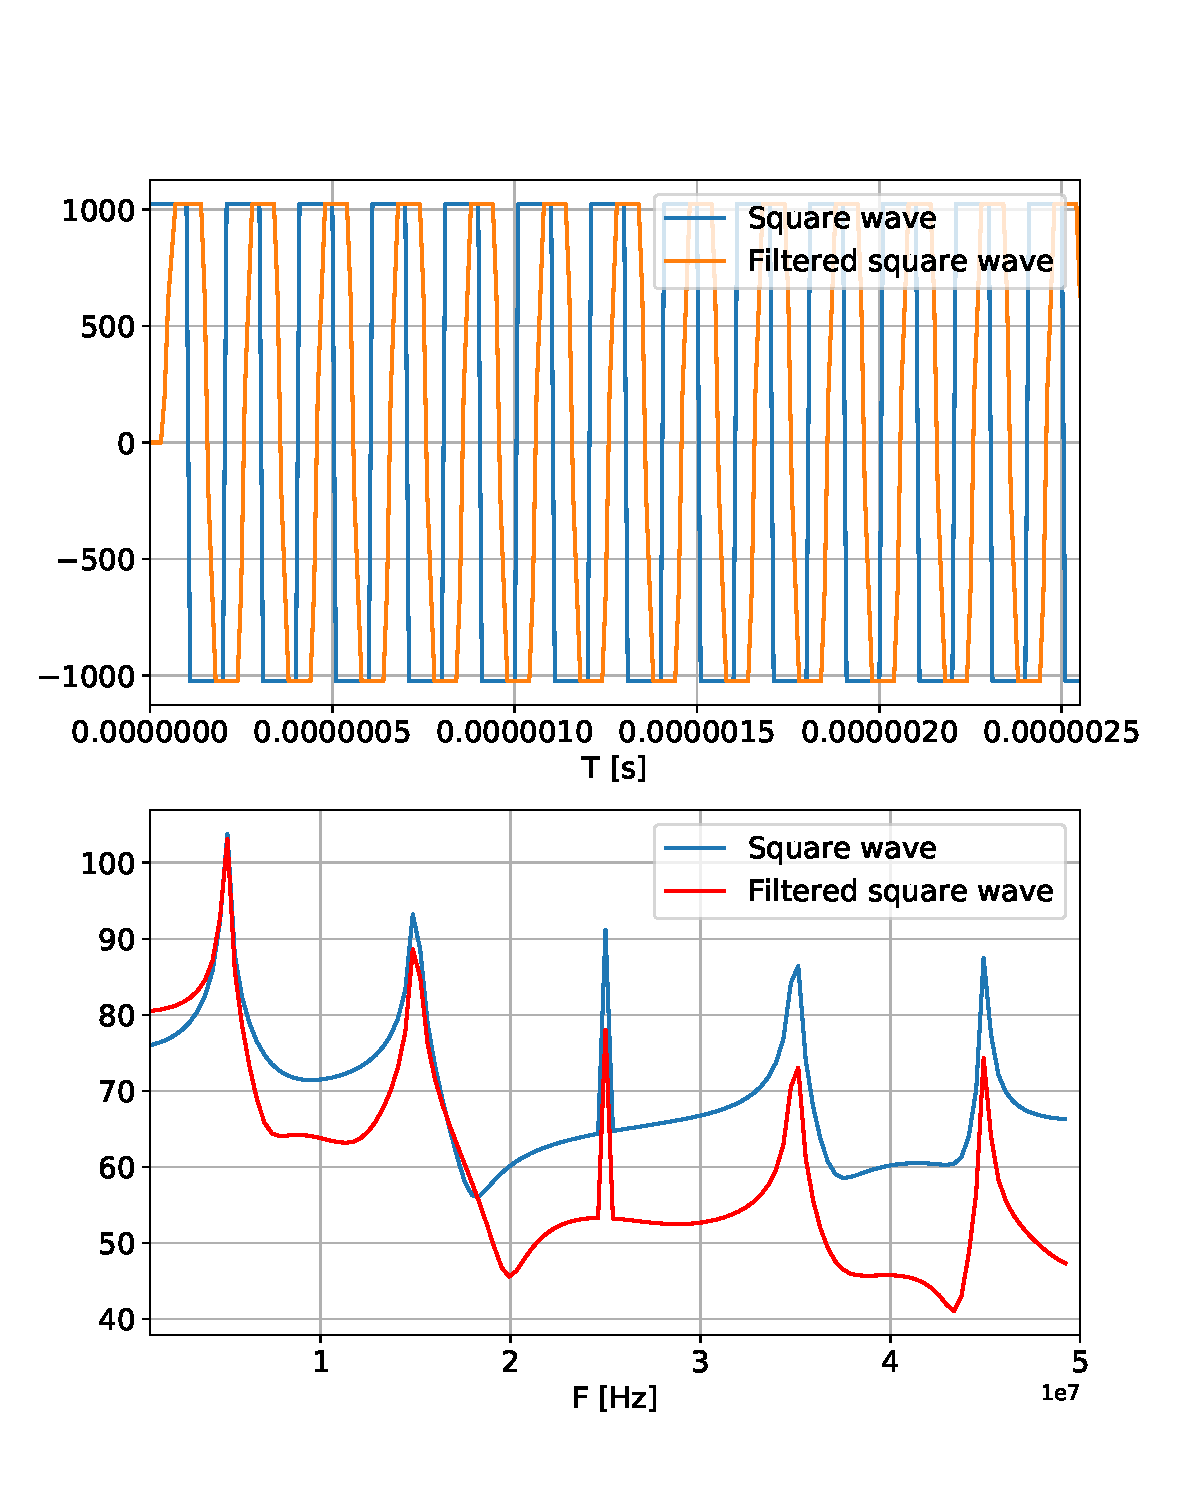
\includegraphics[width=1\linewidth]{./Figure/P20_D50.pdf}
    \end{subfigure}
    \begin{subfigure}{0.49\textwidth}
      \caption{\texttt{PERIOD} = 10, \texttt{DUTY\_CYC} = 50}
      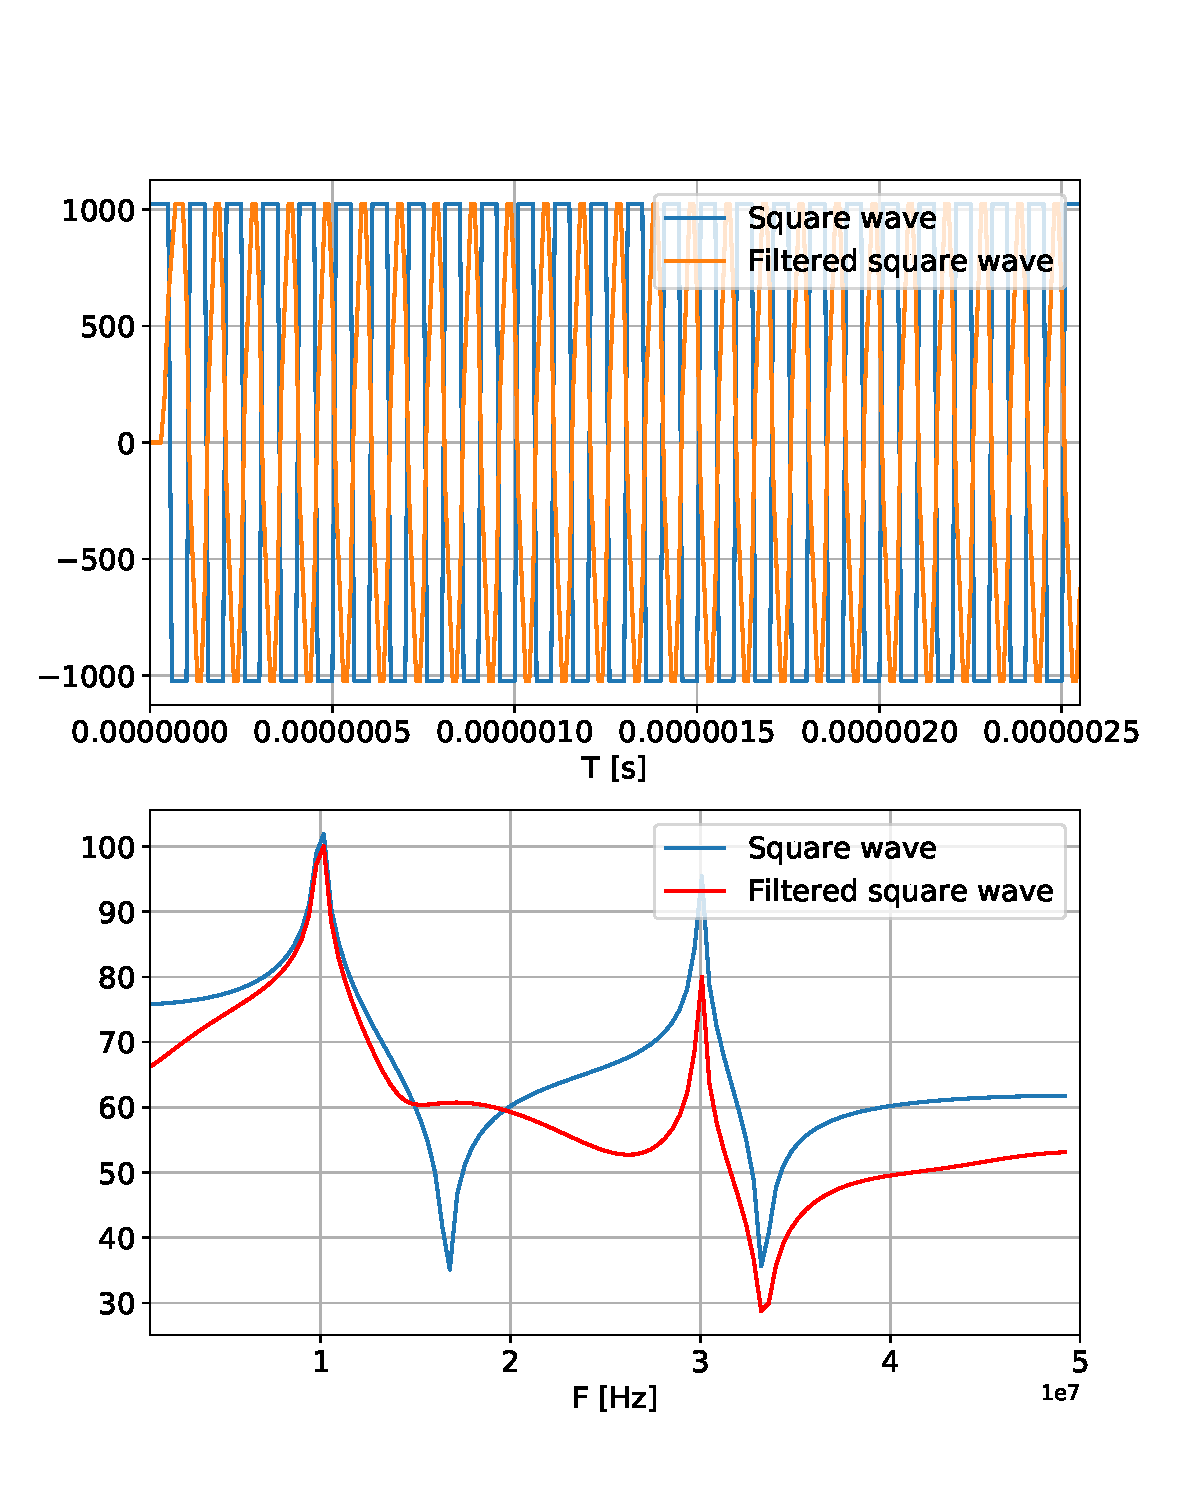
\includegraphics[width=1\linewidth]{./Figure/P10_D50.pdf}
    \end{subfigure}
    \\
    \begin{subfigure}{0.49\textwidth}
      \caption{\texttt{PERIOD} = 20, \texttt{DUTY\_CYC} = 30}
      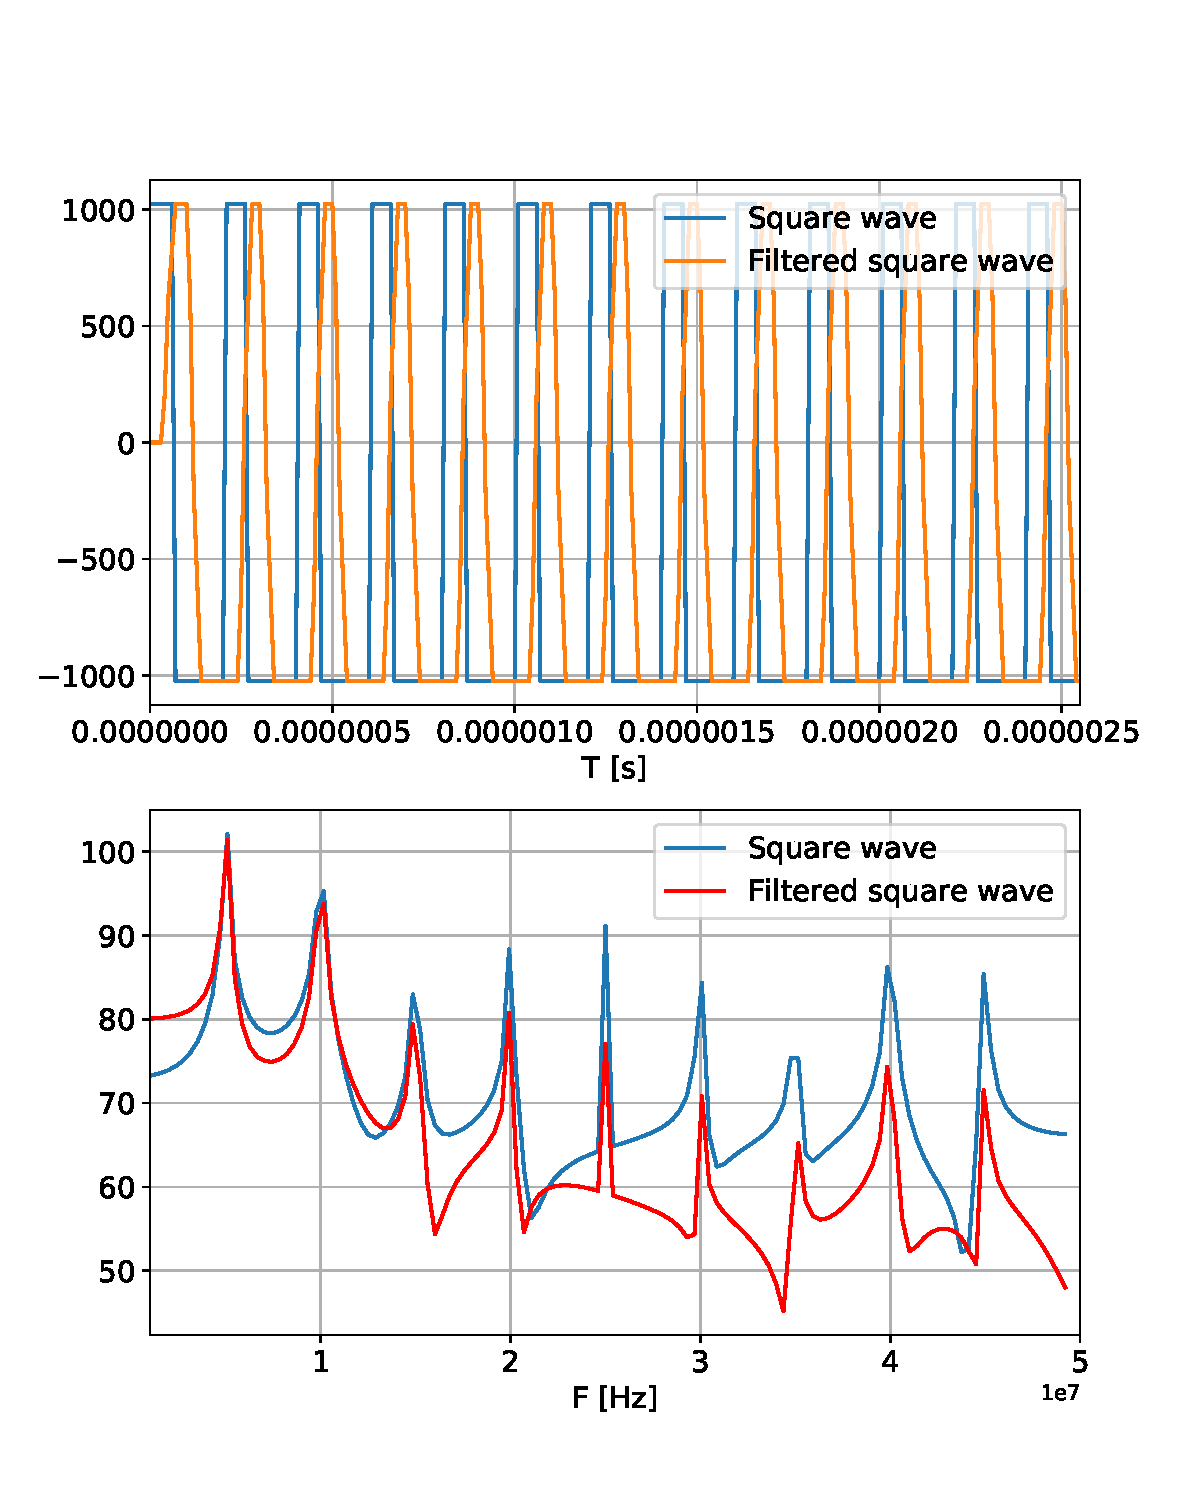
\includegraphics[width=1\linewidth]{./Figure/P20_D30.pdf}
    \end{subfigure}
    \caption{Immagini prodotte dallo script \texttt{final\_project.py} per differenti valori di periodo e duty cycle.}
\end{figure}

\end{document}
